\documentclass{standalone}

\usepackage{tikz}

\usetikzlibrary{positioning, chains, shapes.geometric, fit, shapes, arrows.meta, calc}

\begin{document}

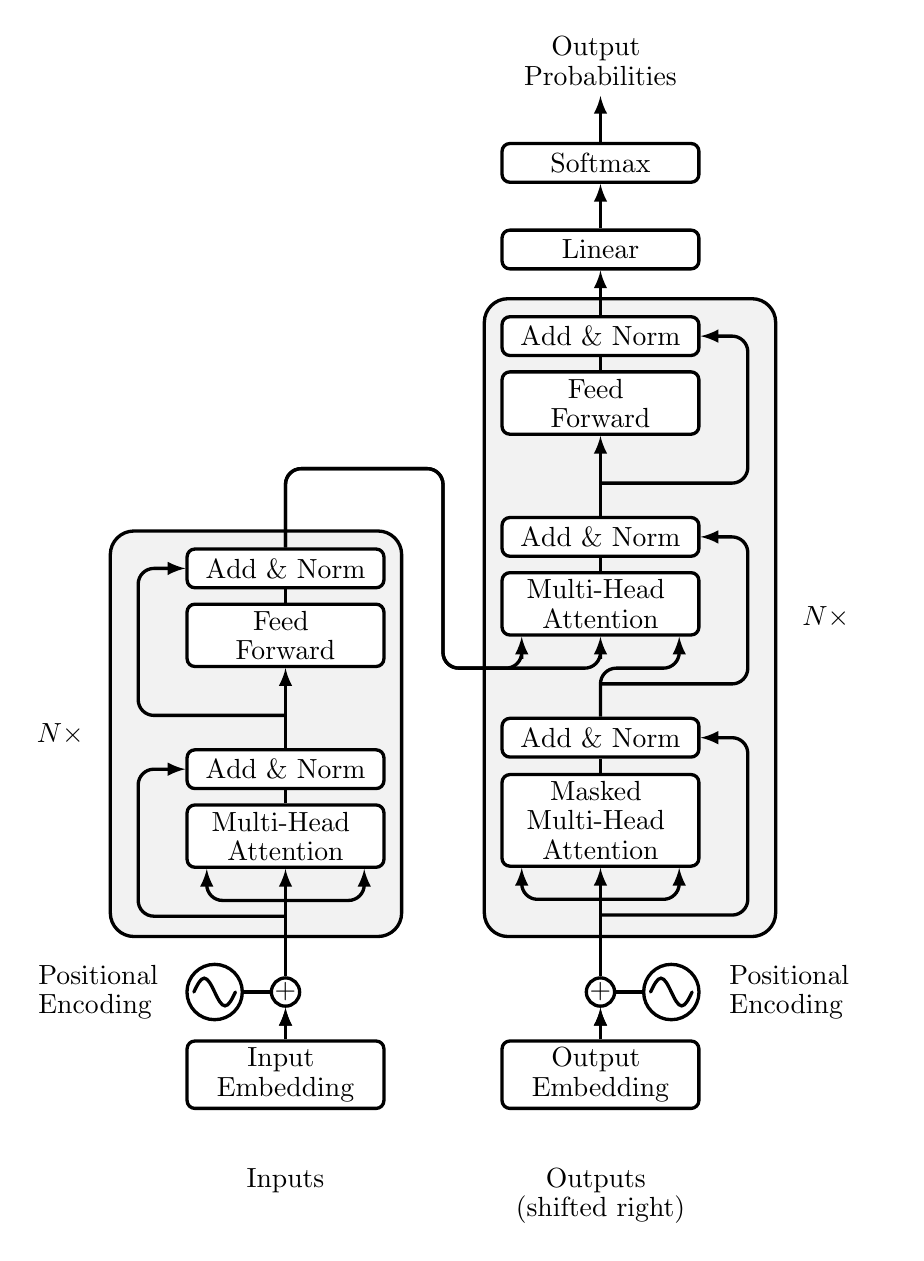
\begin{tikzpicture}[
    >=LaTeX, % Use default LaTeX arrows
    very thick,
    arrow/.style={
        -latex,
        very thick,
        rounded corners=0.2cm
    },
    block/.style={
        rectangle,
        fill=gray!10,
        rounded corners=3mm,
        draw,
        very thick
    },
    layer/.style={
        rectangle,
        fill=white!10,
        rounded corners=1mm,
        inner xsep=0em,
        inner ysep=0.25em,
        minimum height=1.4em,
        align=center,
        text width=2.5cm,
        draw,
        very thick
    },
    input/.style={ % Input or output node
        circle,
        minimum width=2.25em,
        draw,
        fill=gray!10,
        thick
    },
    do path picture/.style={%
        path picture={%
          \pgfpointdiff{\pgfpointanchor{path picture bounding box}{south west}}%
            {\pgfpointanchor{path picture bounding box}{north east}}%
          \pgfgetlastxy\x\y%
          \tikzset{x=\x/2,y=\y/2}%
          #1
        }
    },
    sin wave/.style={do path picture={    
        \draw [line cap=round] (-3/4,0)
        sin (-3/8,1/2) cos (0,0) sin (3/8,-1/2) cos (3/4,0);
        }
    }
]
% Encoder and decoder blocks
\draw[block] (-0.975000, 6.455000) -- (2.725000, 6.455000) -- (2.725000, 1.305000) -- (-0.975000, 1.305000) -- cycle;
\draw[block] (3.775000, 9.405000) -- (7.475000, 9.405000) -- (7.475000, 1.305000) -- (3.775000, 1.305000) -- cycle;

\node[layer] (iemb) at (1.250000,-0.450000) {Input \vspace{-0.05cm} \linebreak Embedding};
\node[layer] (oemb) at (5.250000,-0.450000) {Output \vspace{-0.05cm} \linebreak Embedding};

% Encoder, 1st layer
\node[layer] (add1) at (1.250000,3.430000) {Add \& Norm};
\node[layer] (attn1) at (1.250000,2.580000) {Multi-Head \vspace{-0.05cm} \linebreak Attention};
\draw[] (attn1) -- (add1);

% Decoder, 2nd sub-layer
\node[layer] (add2) at (5.250000,6.380000) {Add \& Norm};
\node[layer] (attn2) at (5.250000,5.530000) {Multi-Head \vspace{-0.05cm} \linebreak Attention};
\draw[] (attn2) -- (add2);

% Decoder 1st sub-layer
\node[layer] (add3) at (5.250000,3.830000) {Add \& Norm};
\node[layer] (attn3) at (5.250000,2.780000) {Masked \vspace{-0.05cm} \linebreak Multi-Head \vspace{-0.05cm} \linebreak Attention};
\draw[] (attn3) -- (add3);

% Encoder 2nd sub-layer
\node[layer] (add4) at (1.250000,5.980000) {Add \& Norm};
\node[layer] (ff1) at (1.250000,5.130000) {Feed \vspace{-0.05cm} \linebreak Forward};
\draw[] (ff1) -- (add4);

% Decoder 3rd sub-layer
\node[layer] (add5) at (5.250000,8.930000) {Add \& Norm};
\node[layer] (ff2) at (5.250000,8.080000) {Feed \vspace{-0.05cm} \linebreak Forward};
\draw[] (ff2) -- (add5);

% Classifier
\node[layer] (linear) at (5.250000,10.030000) {Linear};
\node[layer] (softmax) at (5.250000,11.130000) {Softmax};

% Positional Encoding
\node [circle, draw, sin wave, minimum size=2em] (pe1) at (0.35, 0.6) {};
\node [circle, draw, sin wave, minimum size=2em] (pe2) at (6.15, 0.6) {};
\node[circle, draw, minimum size=0.25em, inner sep=0pt] (sum1) at (1.25, 0.6) {$\boldsymbol{+}$};
\node[circle, draw, minimum size=0.25em, inner sep=0pt] (sum2) at (5.25, 0.6) {$\boldsymbol{+}$};

\draw[arrow] (add1) -- (ff1);
\draw[arrow] (add2) -- (ff2);
\draw[arrow] (add5) -- (linear);
\draw[arrow] (linear) -- (softmax);
\draw[arrow] (iemb) -- (sum1);
\draw[arrow] (sum1) -- (attn1);
\draw[arrow] (oemb) -- (sum2);
\draw[arrow] (sum2) -- (attn3);
\draw[] (sum1) -- (pe1);
\draw[] (sum2) -- (pe2);

\draw[arrow] (ff1.south)++(0, -0.6) -| ($(add4.west) + (-0.6,-0.5)$) |- (add4.west);
\draw[arrow] (attn1.south)++(0, -0.6) -| ($(add1.west) + (-0.6,-0.5)$) |- (add1.west);

\draw[arrow] (attn3.south)++(0, -0.6) -| ($(add3.east) + (0.6,-0.5)$) |- (add3.east);
\draw[arrow] (attn2.south)++(0, -0.6) -| ($(add2.east) + (0.6,-0.5)$) |- (add2.east);
\draw[arrow] (ff2.south)++(0, -0.6) -| ($(add5.east) + (0.6,-0.5)$) |- (add5.east);

\draw[arrow] (attn1.south)++(0, -0.4) -| ($(attn1.south) + (-1,0)$);
\draw[arrow] (attn1.south)++(0, -0.4) -| ($(attn1.south) + (1,0)$);

\draw[arrow] (attn3.south)++(0, -0.4) -| ($(attn3.south) + (-1,0)$);
\draw[arrow] (attn3.south)++(0, -0.4) -| ($(attn3.south) + (1,0)$);

\draw[arrow] (add4.north) |- ($(add4.north) + (1,1)$) -| ($(add4.north) + (2,-1)$) |- ($(attn2.south) + (-1,-0.4)$) -| ($(attn2.south) + (-1,0)$);
\draw[arrow] (add4.north) |- ($(add4.north) + (1,1)$) -| ($(add4.north) + (2,-1)$) |- ($(attn2.south) + (0,-0.4)$) -| ($(attn2.south)$);
\draw[arrow] (add3.north) |- ($(attn2.south) + (0.5,-0.4)$) -| ($(attn2.south) + (1,0)$);

\node[text width=2.5cm, anchor=north, align=center] at (1.25,-1.5) {Inputs};
\node[text width=2.5cm, anchor=north, align=center] at (5.25,-1.5) {Outputs \vspace{-0.05cm} \linebreak (shifted right)};
\node[text width=2.5cm, anchor=south, align=center] (probs) at (5.25,11.98) {Output \vspace{-0.05cm} \linebreak Probabilities};
\node[text width=2cm, anchor=east] at (0.25,0.6) {Positional \vspace{-0.05cm} \linebreak Encoding};
\node[text width=2cm, anchor=west] at (6.75,0.6) {Positional \vspace{-0.05cm} \linebreak Encoding};

\draw[arrow] (iemb) -- (sum1);
\draw[arrow] (oemb) -- (sum2);
\draw[arrow] (softmax) -- (probs);

\node[anchor=east] at (-1.175000,3.880000) {$N\times$};
\node[anchor=west] at (7.675000,5.355000) {$N\times$};

\end{tikzpicture}

\end{document}
